\subsection{\FMoW}\label{sec:app_fmow}

ML models for satellite imagery can enable global-scale monitoring of sustainability and economic challenges, aiding policy and humanitarian efforts in applications such as deforestation tracking~\citep{hansen2013forest}, population density mapping~\citep{tiecke2017population}, crop yield prediction~\citep{wang2020weakly}, and other economic tracking applications~\citep{katona2018parking}.
As satellite data constantly changes due to human activity and environmental processes, these models must be robust to distribution shifts over time.
Moreover, as there can be disparities in the data available between regions,
these models should ideally have uniformly high accuracies instead of only doing well on data-rich regions and countries.

We study this problem on a variant of the Functional Map of the World dataset \citep{christie2018fmow}.

\subsubsection{Setup}

\paragraph{Problem setting.}
We consider a hybrid domain generalization and subpopulation shift problem, where the input $x$ is a RGB satellite image (resized to 224 $\times$ 224 pixels), the label $y$ is one of 62 building or land use categories, and the domain $d$ represents both the year the image was taken as well as its geographical region (Africa, the Americas, Oceania, Asia, or Europe).
We aim to solve both a domain generalization problem across time and improve subpopulation performance across regions.

\paragraph{Data.}
\FMoW is based on the Functional Map of the World dataset~\citep{christie2018fmow}, which collected and categorized high-resolution satellite images from over 200 countries based on the functional purpose of the buildings or land in the image, over the years 2002--2018 (see \reffig{dataset_fmow}).
We use a subset of this data and split it into three time range domains, 2002--2013, 2013--2016, and 2016--2018, as well as five geographical regions as subpopulations (Africa, Americas, Oceania, Asia, and Europe).
For each example, we also provide the timestamp and location coordinates, though our baseline models only use the coarse time ranges and geographical regions instead of these additional metadata.

We use the following data splits:
\begin{enumerate}
    \item \textbf{Training:} 76,863 images from the years 2002--2013.
    \item \textbf{Validation (OOD):} 19,915 images from the years from 2013--2016.
    \item \textbf{Test (OOD):} 22,108 images from the years from 2016--2018.
    \item \textbf{Validation (ID):} 11,483 images from the years from 2002--2013.
    \item \textbf{Test (ID):} 11,327 images from the years from 2002--2013.
\end{enumerate}
The original dataset did not evaluate models under distribution shifts. Our training split is a subset of the original training dataset, filtered for images in the appropriate time range; similarly, our OOD and ID validation splits are subsets of the original validation dataset, and our OOD and ID test splits are subsets of the original test dataset. See \refapp{app_fmow_details} for more dataset details.

The train/val/test data splits contain images from disjoint location coordinates, and all splits contain data from all 5 geographic regions.
The ID and OOD splits within the test and validation sets may have overlapping locations, but have non-overlapping time ranges.
There is a disparity in the number of examples in each region, with Africa and Oceania having the least examples (\reffig{fmow-region-count}); this could be due to bias in sampling and/or a lack of infrastructure and land data in certain regions.

\begin{figure}[tbp]
  \centering
  \begin{subfigure}{0.48\linewidth}
      \centering
      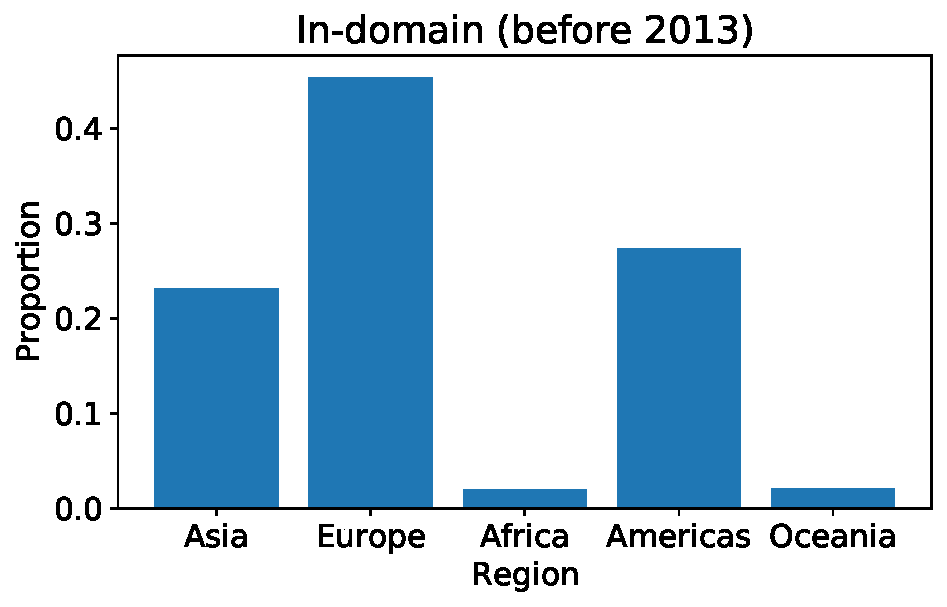
\includegraphics[width=\textwidth]{figures/fmow_region_count_id.pdf}
    \end{subfigure}
    \hfill
    \begin{subfigure}{0.48\linewidth}
      \centering
      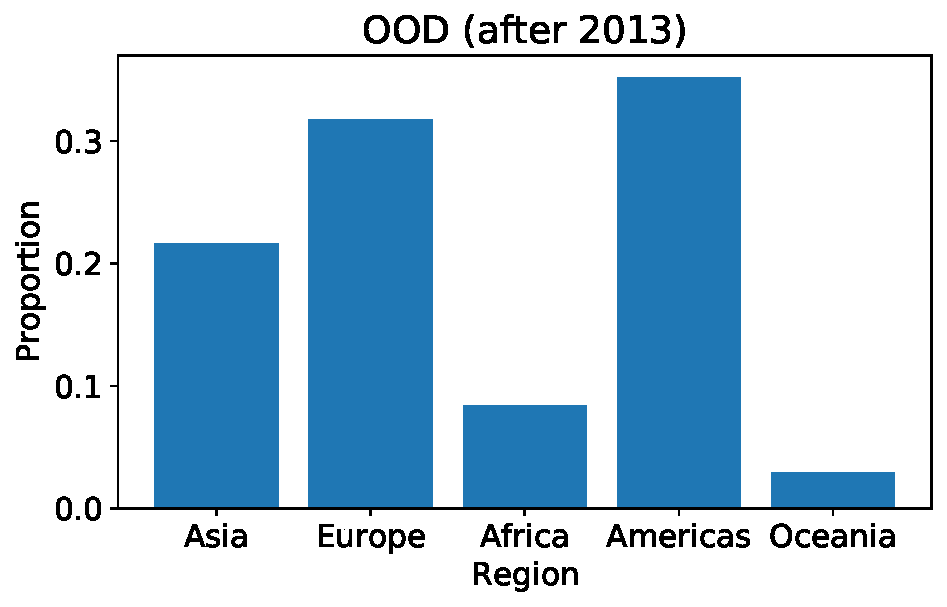
\includegraphics[width=\textwidth]{figures/fmow_region_count_ood.pdf}
    \end{subfigure}
  \caption{Number of examples from each region of the world in \FMoW on the ID vs. OOD splits of the data. There is much less data from Africa and Oceania than other regions.
  }\label{fig:fmow-region-count}
\end{figure}


\paragraph{Evaluation.}
We evaluate models by their average and worst-region OOD accuracies. The former measures the ability of the model to generalize across time, while the latter additionally measures how well models do across different regions/subpopulations under a time shift.

\begin{table*}[tbp]
  \caption{Average and worst-region accuracies (\%) under time shifts in \FMoW. Models are trained on data before 2013 and tested on held-out location coordinates from in-distribution (ID) or out-of-distribution (OOD) test sets.
  ID results correspond to the train-to-train setting.
  Parentheses show standard deviation across 3 replicates.}
  \centering
  \begin{tabular} {l r r r r r}
  \toprule
  & Validation (ID) & Validation (OOD) & Test (ID) & Test (OOD) \\
  \midrule
Average & & & & \\
~~~~ERM        & 61.2 (0.52) & 59.5 (0.37) & \textbf{59.7} (0.65) & \textbf{53.0} (0.55) \\
~~~~CORAL      & 58.3 (0.28) & 56.9 (0.25) & 57.2 (0.90) & 50.5 (0.36) \\
~~~~IRM        & 58.6 (0.07) & 57.4 (0.37) & 57.7 (0.10) & 50.8 (0.13) \\
~~~~Group DRO  & 60.5 (0.36) & 58.8 (0.19) & 59.4 (0.11) & 52.1 (0.50) \\
Worst-region & & & & \\
~~~~ERM        & 59.2 (0.69) & 48.9 (0.62) & \textbf{58.3} (0.92) & \textbf{32.3} (1.25) \\
~~~~CORAL      & 55.9 (0.50) & 47.1 (0.43) & 55.0 (1.02) & 31.7 (1.24) \\
~~~~IRM        & 56.6 (0.59) & 47.5 (1.57) & 56.0 (0.34) & 30.0 (1.37) \\
~~~~Group DRO  & 57.9 (0.62) & 46.5 (0.25) & 57.8 (0.60) & 30.8 (0.81) \\
  \bottomrule
\end{tabular}
\label{table:fmow-leaderboard}
\end{table*}



\begin{table*}[!h]
  \caption{The regional accuracies of models trained on data before 2013 and tested on held-out locations from ID ($< 2013$) or OOD ($\geq 2016$) test sets in \FMoW. ID results correspond to the train-to-train setting. Standard deviations over 3 trials are in parentheses.}
  \centering
\begin{tabular} {l r r r r r r}
\toprule
& Asia & Europe & Africa & Americas & Oceania & Worst region\\
\midrule
OOD Test & & & & & & \\
~~~~ERM & 55.4 (0.95) & 55.6 (0.53) & 32.3 (1.25) & 55.7 (0.48) & 59.1 (0.85) & 32.3 (1.25)  \\
~~~~CORAL & 52.4 (0.96) & 52.6 (0.82) & 31.7 (1.24) & 53.3 (0.27) & 56.0 (2.02) & 31.7 (1.24)\\
~~~~IRM & 52.9 (0.73) & 53.9 (0.28) & 30.0 (1.37) & 53.7 (0.51) & 55.0 (2.22) & 30.0 (1.37)\\
~~~~Group DRO  & 54.7 (0.52) & 55.1 (0.39) & 30.8 (0.81) & 54.6 (0.48) & 58.5 (1.65) & 30.8 (0.81) \\
ID Test & & & & & & \\
~~~~ERM & 58.9 (1.19) & 58.4 (0.81) & 69.1 (2.64) & 61.4 (0.35) & 69.9 (0.53) & 58.3 (0.92)\\
~~~~CORAL & 56.6 (1.35) & 55.0 (1.02) & 69.2 (2.92) & 59.7 (0.83) & 70.8 (2.53) & 55.0 (1.02)\\
~~~~IRM & 56.9 (0.62) & 56.0 (0.34) & 69.7 (2.16) & 59.7 (0.49) & 68.3 (2.00) & 56.0 (0.34)\\
~~~~Group DRO  & 58.7 (0.33) & 57.9 (0.74) & 69.2 (0.28) & 61.1 (0.57) & 68.8 (2.38) & 57.8 (0.60) \\
\bottomrule
\end{tabular}
\label{table:fmow-region}
\end{table*}


\begin{table*}[!h]
  \caption{Mixed-to-test comparison for ERM models on \FMoW.
  In the official setting, we train on ID examples (i.e., data from 2002--2013),
  whereas in the mixed-to-test ID setting, we train on ID + OOD examples (i.e., the same amount of data but half from 2002--2013 and half from 2013--2018, using a held-out set of data from 2013--2018).
  In both settings, we test on the same Test (ID) data (from 2002--2013) and Test (OOD) data (from 2013--2018) described in the official split.
  Models trained on the official split degrade in performance under the time shift, especially on the last year (2017) of the test data, and also fare poorly on the subpopulation shift, with low worst-region accuracy.
  Models trained on the mixed-to-test split have higher OOD average and last year accuracy and much higher OOD worst-region accuracy.
  Standard deviations over 3 trials are in parentheses.}
  \centering
  \begin{tabular} {l l r r r r r}
  \toprule
  & & \multicolumn{2}{c}{Test (ID)} & \multicolumn{3}{c}{Test (OOD)} \\
  Setting & Algorithm & Average & Worst-region & Average & Last year & Worst-region\\
  \midrule
  Official & ERM & 59.7 (0.65) & 58.3 (0.92) & 53.0 (0.55) & 48.1 (1.20) & 32.3 (1.25) \\
  Mixed-to-test & ERM & 59.0 (0.47) & 56.9 (0.80) & 57.4 (0.27) & 54.3 (0.22) & 48.6 (0.89)\\
  \bottomrule
  \end{tabular}
  \label{table:fmow-compare}
\end{table*}

\paragraph{Potential leverage.}
\FMoW considers both domain generalization across time and subpopulation shift across regions. As we provide both time and region annotations, models can leverage the structure across both space and time to improve robustness.
For example, one hypothesis is that infrastructure development occurs smoothly over time. Utilizing this gradual shift structure with the timestamp metadata may enable adaptation across longer time periods~\citep{kumar2020gradual}.
The data distribution may also shift smoothly over spatial locations, and so enforcing some consistency with respect to spatial structure may improve predictions~\citep{rolf2020post,jean2018ssdkl}.
Furthermore, to mitigate the fact that some regions (e.g., Africa) have less labeled data, one could potentially transfer knowledge of other regions with similar economies and infrastructure. The location coordinate metadata allows for transfer learning across similar locations at any spatial scale.

\subsubsection{Baseline results}
\paragraph{Model.} For all experiments, we follow \citet{christie2018fmow} and use a DenseNet-121 model~\citep{huang2017densely} pretrained on ImageNet and with no $L_2$ regularization.
We use the Adam optimizer \citep{kingma2014adam} with an initial learning rate of $10^{-4}$ that decays by 0.96 per epoch, and train for 50 epochs for with early stopping and with a batch size of 64.
All reported results are averaged over 3 random seeds.

\paragraph{ERM results and performance drops.}
In the train-to-train comparison, Table~\ref{table:fmow-compare} shows that average accuracy drops by 6.7\% when evaluated on the OOD test set ($\geq 2016$) compared to the ID test set setting.
The drop in average accuracy is especially large (11.6\%) on images from the last year of the dataset (2017), furthest in the future from the training set.
In addition, there is a substantial 26.0\% drop in worst-region accuracy, with the model performing much worse in Africa than other regions (Table~\ref{table:fmow-region}).

We also ran a mixed-to-test comparison where we mixed in some data from the OOD period (2013--2018) into the training set, while keeping the overall training set size constant.
A model trained on this mixed split had a much smaller drop in performance under the time and region shifts (Table~\ref{table:fmow-compare}).
While the magnitude of the ID-OOD gap in worst-region accuracy shrinks from 26.0\% in the train-to-train setting to 16.3\% in the mixed-to-test setting, the gap remains significant, implying that the drop in performance is largely due to the distribution shift across time and region instead of  a change in the intrinsic difficulty of the OOD data.

\paragraph{Additional baseline methods.}
We compare ERM against CORAL, IRM, and Group DRO, using examples from different years as distinct domains. Table~\ref{table:fmow-leaderboard} shows that many of these methods are comparable or worse than ERM in terms of both ID and OOD test performance.
As with most other datasets, our grid search selected the lowest values of the penalty weights for CORAL ($\lambda = 0.1$) and IRM ($\lambda = 1$).


\paragraph{Discussion.}
Intriguingly, a large subpopulation shift across regions only occurs with a combination of time and region shift.
This is corroborated by the mixed-split region shift results (Table~\ref{table:fmow-compare}), which do not have a time shift between training and test sets, and correspondingly do not display a large disparity in performance across regions.
This drop in performance may be partially due to label shift:
from Figure~\ref{fig:fmow-classfreqs}, we see that the label distributions between Africa and other  regions are very different, e.g., with a large drop in recreational facilities and a sharp increase in single residential units.
We do not find a similarly large label shift between $<2013$ and $\geq 2013$ splits of the dataset.

\begin{figure*}[tbp]
  \centering
  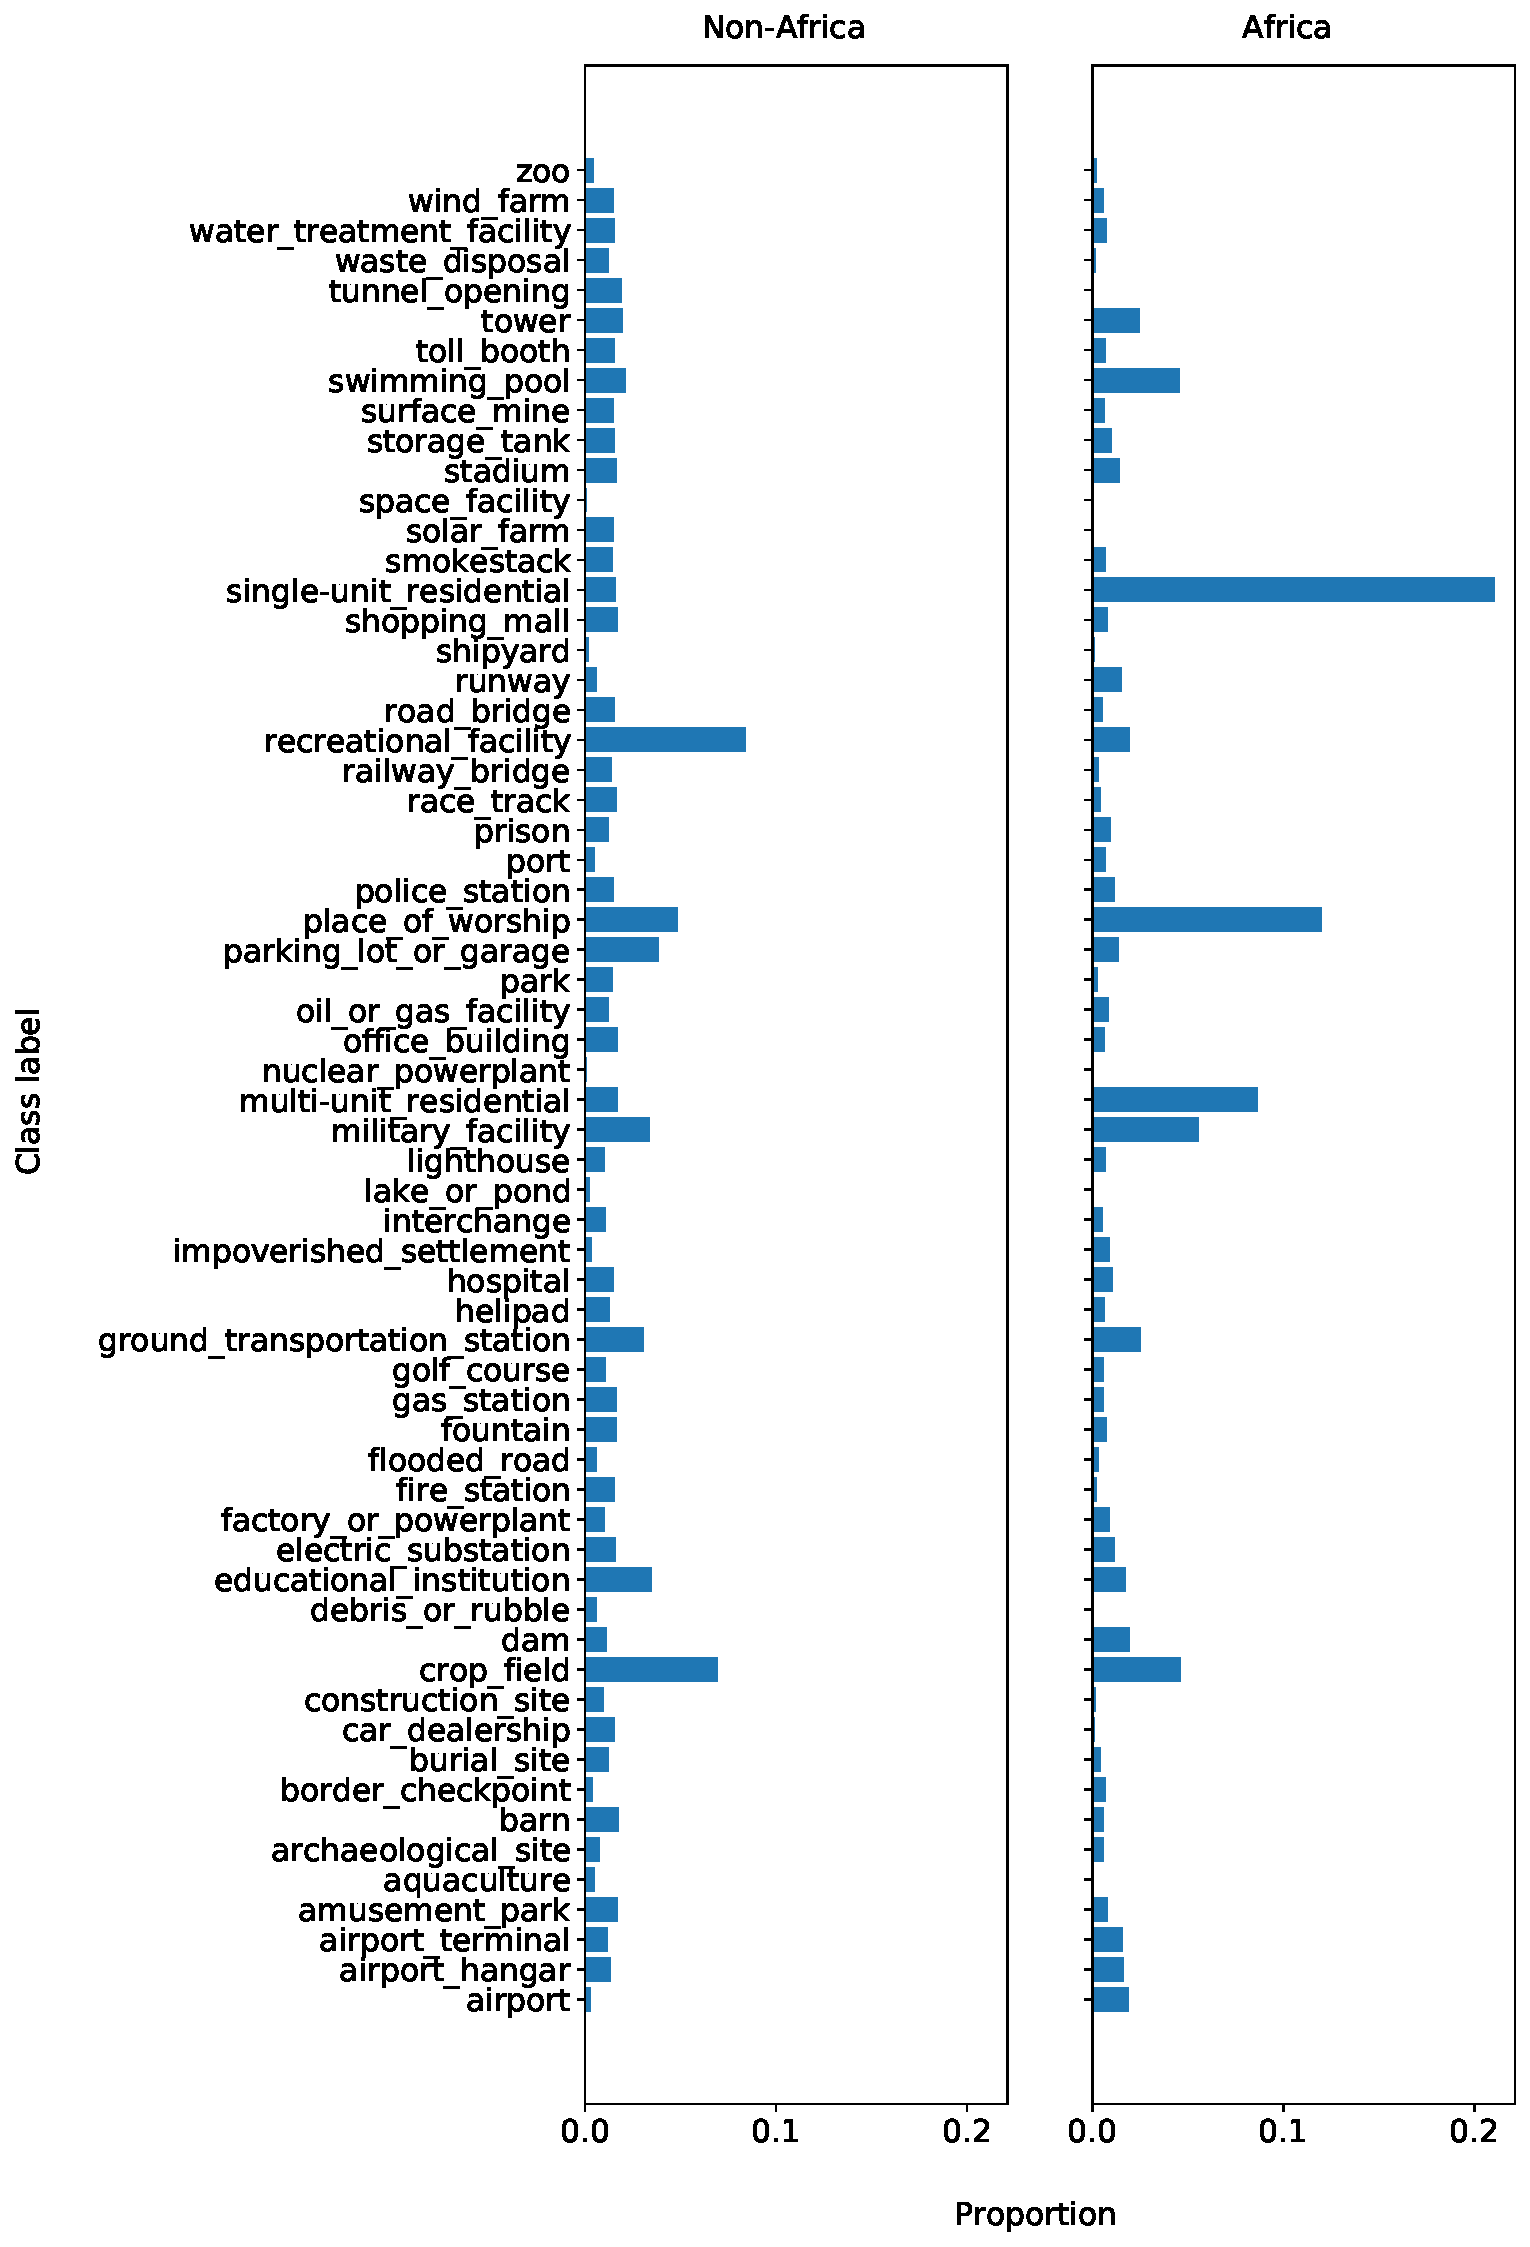
\includegraphics[width=0.9\textwidth]{figures/fmow_combined_classfreqs.pdf}
  \caption{Number of examples from each category in \FMoW in non-African and African regions. There is a large label shift between non-African regions and Africa.}\label{fig:fmow-classfreqs}
\end{figure*}


Despite having the smallest number of training examples (Figure~\ref{fig:fmow-region-count}), the baseline models do not suffer a drop in performance in Oceania on validation or test sets (Table~\ref{table:fmow-region}). We hypothesize that infrastructure in Oceania is more similar to regions with a large amount of data than Africa.
In contrast, Africa may be more distinct and may have changed more drastically over 2002-2018, the time extent of the dataset.
This suggests that the subpopulation shift is not merely a function of the number of training examples.

We note that our dataset splits can separate on particular factors such as the introduction of new sensors, which is natural with progression over time. For example, the WorldView-3 sensor came online in 2014. Future work should look into the role of auxiliary factors such as new sensors that are associated with time but may be controllable. We did not find a sharp difference in performance due to the introduction of WorldView-3; we found that the performance decays gradually over time, suggesting that the performance drop comes from other factors.

As with \PovertyMap, there are important ethical considerations associated with remote sensing applications,
e.g., around surveillance and privacy issues, as well as the potential for systematic biases that negatively affect particular populations.
As an example of the latter, the poor model performance on satellite images from Africa that we observe in \FMoW raises issues of bias and fairness.
With regard to privacy, we note that the image resolution in \FMoW is lower than that of other public and easily-accessible satellite data such as that from Google Maps.
We refer interested readers to the UNICEF discussion paper by \citet{berman2018ethical} for a more in-depth discussion of the ethics of remote sensing especially as it pertains to development and humanitarian endeavors.


\subsubsection{Broader context}
Recognizing infrastructure and land features is crucial to many remote sensing applications. For example, in crop land prediction~\cite{wang2020weakly}, recognizing gridded plot lines, plot circles, farm houses, and other visible features are important in recognizing crop fields. However, farming practices and equipment evolve over time and vary widely across the world, requiring both robust object recognition and synthesis of their different usage patterns.

Although the data is typically limited, we desire generalization on a global scale without requiring frequent large-scale efforts to gather more ground-truth data.
It is natural to have labeled data with limited temporal or spatial extent since ground truth generally must be verified on the ground or requires manual annotations from domain experts (i.e., they are often hard to be crowdsourced). A number of existing remote sensing datasets have limited spatial or temporal scope, including the UC Merced Land Use Dataset~\citep{yang2010landuse}, TorontoCity~\citep{wang2017torontocity}, and SpaceNet~\citep{digitalglobe2016spacenet}.
However, works based on these datasets generally do not systematically study shifts in time or location.

\subsubsection{Additional details}\label{sec:app_fmow_details}

\paragraph{Data processing and modifications to the original dataset.}
The \FMoW dataset is derived from~\citet{christie2018fmow}, which collected over 1 million satellite images from over 200 countries over 2002-2018.
We use the RGB version of the original dataset, which contains 523,846 total examples, excluding the multispectral version of the images.
Methods that can utilize a sequence of images can group the images from the same location across multiple years together as input, but we consider the simple formulation here for our baseline evaluation.

The original dataset from~\citet{christie2018fmow} is provided as a set of hierarchical directories with JPEG images of varying sizes.
To reduce download times and I/O usage, we resize these images to 224 $\times$ 224 pixels, and then store them as PNG images.
We also collect all the metadata into CSV format for easy processing.

The original dataset is posed as a image time-series classification problem, where the model has access to a sequence of images at each location. For simplicity, we treat each image as a separate example, while making sure that the data splits all contain disjoint locations. We use the train/val/test splits from the original dataset, but separate out two OOD time segments: we treat the original validation data from 2013-2016 as OOD val and the original test data from 2016-2018 as OOD test. We remove data from after 2013 from the training set, which reduces the size of the training set in comparison to the original dataset.


\paragraph{Additional challenges in high-resolution satellite datasets.}
Compared to \PovertyMap, \FMoW contains much higher resolution images (sub-meter resolution vs. 30m resolution) and contains a larger variety of viewpoints/tilts, both of which could present computational or algorithmic challenges. For computational purposes, we resized all images to $224\times 224$ (following~\citet{christie2018fmow}), but raw images can be thousands of pixels wide. Some recent works have tried to balance this tradeoff between viewing overall context and the fine-grained detail~\citep{uzkent2020zoom,kim2016multiresolution}, but how best to do this is an open question. \FMoW also contains additional information on azimuth and cloud cover which could be used to correct for the variety in viewpoints and image quality.
